\documentclass[final]{these-ISSS}

\usepackage{mesmacros}

%%%%%%%%%%%%%%%%%%%%%%%%%%%%%%%%%%%%%%%%%%%%%%%
%%%%%%%%%%%%%%%%%%%%%%%%%%%%%%%%%%%%%%%%%%%%%%% 
\titre{Pourquoi les macarons de Ladurée sont-ils si bons ?}
%\soustitre{C'est si bon}
\title{Why Ladurée macarons are so good?}
\firstname{Pierre}
\lastname{Hermé}
%\laboratoire{} %Déclaration du nom du labo si ce n'est pas l'I3S
%\cotutelle{Université de la Pâtisserie} % Ajouter une cotutelle si elle existe
%\cotutellelogo{Pastry_Bag.png}
\date{} % Mettre la date de soutenance
\discipline{Pâtisserie} % Informatique par défaut
%\cofinanceurslogo{Pastry_Bag.png, Pastry_Bag.png, Pastry_Bag.png}
%\hdr

%%%%%%%%%%%%%%%%%%%%%%%%%%%%%%%%%%%%%%%%%%%%%%%
%%%%%%%%%%%%%%%%%%%%%%%%%%%%%%%%%%%%%%%%%%%%%%%

\usepackage[pdftex,
            bookmarks=true,
            bookmarksnumbered=true,
            breaklinks=true,
            colorlinks=true,
            citecolor=bleu]{hyperref}
            
\usepackage{minitoc}
\dominitoc[n]
\dominilof
\dominilot
%\setcounter{minitocdepth}{3}
\renewcommand{\mtctitle}{Sommaire}

%%%%%%%%%%%%%%%%%%%%%%%%%%%%%%%%%%%%%%%%%%%%%%%
%%%%%%%%%%%%%%%%%%%%%%%%%%%%%%%%%%%%%%%%%%%%%%%


\begin{document}
  \pagenumbering{roman}  

%%------------------------------------------------------------------- Le jury
\begin{jury}[Paul \Nom{Bocuse}, Grand chef cuisinier/L'Auberge du Pont de Collonges]%% Mettre ici le nom du président
%% Autant de lignes \rapporteur que nécessaire
%% Autant de lignes \examinateur que nécessaire
  \rapporteur{Patrick \Nom{Lenôtre}}{Chef de cuisine}{Pavillon des Princes, Paris}
  \rapporteur{Christophe \Nom{Michalak}}{Chef pâtissier}{l'Hôtel Plaza-Athénée, Paris}
  \examinateur{Cédric \Nom{Grolet}}{Chef pâtissier}{Le Meurice}
  \invite{Michel \Nom{Guérard}}{Cuisinier}{Les Prés d'Eugénie}
  \directeur{Jean-Paul \Nom{Hévin}}
  \codirecteur{Antoine \Nom{Santos}}
  \coencadrant{Laurent \Nom{Duchêne}}
\end{jury}

%%-----------------------------------------------------------------------------

\maketitle

\begin{dedicace}
  À toi lecteur <3 :*
\end{dedicace}

\cleardoublepage
%%------------------------------------------------ Le résumé et les mots-clés -
\begin{ResumeMotsCles}
%% Résumé en français : pas plus de 2000 caractères
\begin{resume}
Les macarons c'est bon par nature, c'est le propre même du macaron que d'être bon. Au vue de l'affluence constante aux divers magasins Ladurée on peut supposer que les macarons qu'on y trouve sont meilleurs qu'ailleurs. Cette thèse vise à donner des idées et pistes sur le pourquoi du comment que les macarons de Ladurée sont si bons.
\end{resume}

%% Résumé en anglais : pas plus de 2000 caractères
\begin{abstract}
Macarons are so good.
\end{abstract}

%% Mots-clés en français
\motscles{Pâtisserie, Macaron, Ladurée.}
%% Mots-clés en anglais
\keywords{Pastry, Macaron, Ladurée.}
\end{ResumeMotsCles}

%%%%%%%%%%%%%%%%%%%%%%%%%%%%%%%%%%%%%%%%%%%%%
\begin{remerciements}
Merci !
\end{remerciements}
%%%%%%%%%%%%%%%%%%%%%%%%%%%%%%%%%%%%%%%%%%%%%%



\tableofcontents

\mainmatter

% !TEX root = ../sommaire.tex

\chapter{Introduction}

Cette classe \LaTeX est basée sur la classe \texttt{these-LINA} écrite par Frédéric Goualard. La classe a été modifiée pour correspondre au modèle de thèse demandé par l'ED STIC de l'Université Côte d'Azur.

Pour les autres ED, il suffit de supprimer le fichier \texttt{visuel.jpg} dans le dossier \texttt{img/} et de renommer le visuel correspondant à l'ED en \texttt{visuel.jpg}.

\section{Organisation}
  
  Pour compiler ce document vous pouvez utiliser le \texttt{Makefile}.

  \subsection{Fichier principal et informations}
  Le fichier principal est le fichier \texttt{sommaire.tex}, la classe du document est \texttt{these-ISSS}. 
  Différentes options sont possibles :
  \begin{itemize}
    \item \texttt{draft} pour une version brouillon du manuscrit, les liens sont désactivés et en noir, et les étiquettes des références sont affichées ;
    \item \texttt{revision} qui ajoute à chaque première page de chapitre la date et l'heure de la dernière compilation en pied de page ;
    \item \texttt{gray} pour une version en grayscale du manuscrit ;
    \item \texttt{final} (par défaut) pour la version finale du manuscrit ;
    \item \texttt{oneside} pour une impression recto et \texttt{twoside} (par défaut) pour une impression recto-verso ;
    \item \texttt{notitlepage} pour un manuscrit sans page de titre et \texttt{titlepage} (par défaut) avec page de titre.
  \end{itemize}
  
  Le titre du document ainsi que les informations correspondant au laboratoire, une co-tutelle ou les co-financeurs se trouvent dans le fichier \texttt{titreEtInfos.tex}.
  
  Les informations relatives au jury, au directeur, co-directeur et co-encadrant se trouvent dans le fichier \texttt{jury.tex}.
  
  Le résumée et les mots-clés en français et en anglais se trouvent dans le fichier \texttt{resume.tex}.
  
  \subsection{Les chapitres}
  À l'exception des remerciements et des notations, chaque chapitre a son dossier. 
  Ce n'est pas nécessaire mais c'est plus facile pour s'y retrouver après, et dans chaque dossier il y a le fichier principal, et il peut y avoir d'autre fichiers ou dossiers (par exemple un dossier \texttt{img/}).
  
  Les chapitres sont ajoutés aux document principal à l'aide des macros \verb|\input| ou \verb|\import|. À noter que la macro \verb|\include| ajoute forcément une nouvelle page et ne permet pas des inclusions en cascades, son utilisation est à éviter.
  
  \subsection{Les paquets}
  Les ajouts de paquets sont dans le fichier \texttt{mesmacros.sty}. Vous pouvez supprimer ou ajouter dans ce fichier d'autres paquets. 
  
  Ce fichier utilise les fichiers suivant :
  \begin{itemize}
    \item \texttt{francisation.sty} dans lequel se trouvent les traductions des différents noms de section ou listes ;
    \item \texttt{couleurs.sty} dans lequel se trouvent des couleurs, et dans lequel vous pouvez ajouter des couleurs ;
    \item \texttt{theoremNames.sty} dans lequel se trouvent les définitions de théorèmes ;
    \item \texttt{theoremList.sty} dans lequel se trouve le code pour générer des listes de théorèmes, utilisé pour générer la liste des définitions et la liste des exemples à la fin de ce document ;
    \item \texttt{algo.sty} pour les algorithmes en français avec le package \texttt{algorithmic} et \texttt{colorationSyntaxique.sty} pour la coloration syntaxique des algorithmes avec le package \texttt{lstlistings}.
  \end{itemize}

\section{Citations}

Dans ce document on a créé 3 bibliographie :
\begin{itemize}
  \item la bibliographie pour les publications personnelles,
  \item la bibliographie pour les pages web,
  \item et la bibliographie générale.
\end{itemize}

Elles sont définies au début du fichier \texttt{sommaire.tex}.

\begin{framed}
\begin{verbatim}
% Biblio pour les pages webs
\newcites{web}{Pages web}
% Biblio pour mes publications
\newcites{mine}{Mes publications}
\end{verbatim}\vspace{-0.5em}
\end{framed}

On utilise pour cela le package \texttt{multibib}, vous pouvez ajouter les votre ou renommer celles existantes, il ne faut pas oublier de modifier le fichier \texttt{Makefile} pour compiler les nouvelles bibliographies ou supprimer la compilation de celles que vous n'utiliser pas.

\paragraph{Les publications dans la bibliographie générale} doivent être citées avec la macro \texttt{\textbackslash cite\{key\}}.

\begin{framed}
\noindent\cite{T2012}\vspace{-0.5em}
\begin{verbatim}\cite{T2012}\end{verbatim}\vspace{-0.75em}
\end{framed}

\paragraph{Les publications pour la section pages web} doivent être citées avec la macro \texttt{\textbackslash citeweb\{key\}}.

\begin{framed}
\noindent\citeweb{AC9} \vspace{-0.5em}
\begin{verbatim}\citeweb{AC9}\end{verbatim}\vspace{-0.75em}
\end{framed}

\paragraph{Les publications pour la section correspondant à vos publications} doivent être citées avec la macro \texttt{\textbackslash citemine\{key\}}.

\begin{framed}
\noindent\citemine{DHHS2011} \vspace{-0.5em}
\begin{verbatim}\citemine{DHHS2011}\end{verbatim}\vspace{-0.75em}
\end{framed}

Pour référencer vos publications par la suite, vous pouvez utiliser la macro \texttt{\textbackslash cite} ou la macro \texttt{\textbackslash citemine}.
Si vous souhaitez que votre publication apparaisse dans la bibliographie générale à la fin du manuscript vous pouvez soit la citer avec \texttt{\textbackslash cite} ou l'insérer avec \texttt{\textbackslash nocite}. \nocite{DHHS2011} 

Attention si vous utilisez un style de bibliographie numérotant les références, vous aurez des problèmes de numérotation si une publication est à la fois citée en utilisant la macro \texttt{\textbackslash cite} et la macro \texttt{\textbackslash citemine}.


Chaque bibliographie peut ensuite être affichée en utilisant les lignes suivantes :

\begin{framed}
\begin{verbatim}\bibliographystyle<s>{apalike}
\bibliography<s>{biblio}
\end{verbatim}\vspace{-0.5em}
\end{framed}

où \verb|<s>| correspond à la bibliographie que l'on veut afficher.


\section{Exemples d'utilisation}

Des exemples d'utilisation des différents paquets sont présents dans ce document.


Des citations pour compléter les bibliographies \citemine{HHSD2011,HHSD2012}, \citeweb{AC9}.
 

  
\renewcommand{\bibtitle}{\section*{\refname}}
\bibliographystylemine{apalike}
\bibliographymine{biblio}



% !TEX root = sommaire.tex
\Chapter{Notations}

\section*{P\^atisserie}

\begin{tabular}{p{2cm} p{11.5cm}}
  \hline
  $\mathcal{D}$ & l'ensemble des donuts\\
  $\mathcal{M}$ & l'ensemble des macarons\\
  $d_i$ & le donut $i$\\
  $m_i$ & le macaron $i$\\
  \hline
\end{tabular}

\section*{Viennoiserie}

\begin{tabular}{p{2cm} p{11.5cm}}
  \hline
  $\mathcal{V}$ & l'ensemble des viennoiseries\\
  $\mathcal{C}$ & l'ensemble des croissants\\
  $v_i$ & la viennoiserie $i$\\
  $c_i$ & le croissant $i$\\
  \hline
\end{tabular}


\Part{État de l'art}
% !TEX root = ../sommaire.tex

\chapter{La Pâtisserie}

\chapres{Dans ce chapitre nous présentons l'histoire de la pâtisserie et plus particulièrement l'histoire de la pâtisserie française et du macaron.}{In this chapter we present the history of pastry and more particularly the history of french pastry and macaron.}

% !TEX root = ../sommaire.tex

\section{La pâtisserie de la préhistoire à aujourd'hui}

Comme chacun sait la pâtisserie a toujours existé, même les hommes et femmes préhistoriques aimaient finir leurs repas sur une note sucrée.

\subsection{Les premiers gâteaux}


\subsubsection{La première tarte}

Rappelons d'abord la définition de la tarte telle que donnée dans \cite{S2012}.

\begin{definition}[Tarte]
  Une tarte, c'est comme un donuts mais sans trous et avec des fois des fruits dessus.
\end{definition}

\begin{example}[Tarte]
  La tarte aux citrons et une tarte.
\end{example}

\begin{remark}
  Notons que la tarte au chocolat est aussi une tarte par contre le mille-feuilles n'est pas une tarte.
\end{remark}

Après de très nombreux travaux on peut aujourd'hui affirmer que la première tarte était une tarte aux citrons, et vous devez nous croire parce qu'on porte des lunettes de soleil \cite{C2012}.

\subsubsection{Le premier éclair}

\subsubsection{Le premier flan}

\subsubsection{La première religieuse}


\subsection{évolution de la pâtisserie au cours du temps}

\subsection{L'arrivée du Macaron}

\subsection{Conclusion}

\section{La pâtisserie dans le monde}


\subsection{Pâtisserie suédoise}
Les suédois font \emph{fika} pour le plaisir de tous.

\subsection{Pâtisserie orientale}
Toutes ces pâtisseries très sucrées à la pistache qui sont très très bonnes.

\subsection{Pâtisserie anglaise}
Non c'est une blague :) \cite{F2011}

\subsection{Conclusion}



\section{Synthèse}


\subsection{La place du macaron dans le monde}

\subsection{Analyse}

% !TEX root = ../sommaire.tex

\chapter{Les macarons c'est bon}

\chapintro{En fait, j'en ai marre de mettre des résumés en anglais.}

%%%%%%%%%%%%%%%%%%%%%%%%%%%%%
\section{Introduction}
%%%%%%%%%%%%%%%%%%%%%%%%%%%%%

%%%%%%%%%%%%%%%%%%%%%%%%%%%%%
\section{Les macarons}
%%%%%%%%%%%%%%%%%%%%%%%%%%%%%
\begin{definition}[Macaron]
  Les macarons c'est de petits gâteaux à base de meringue qui sont très bons.
  \label{def:macaron}
\end{definition}

\begin{proposition}
  Les macarons c'est bon.
\end{proposition}

\begin{proof}
  Montrons que macarons $\Leftrightarrow$ bon
  
  \begin{myproof}[macaron $\Rightarrow$ bon]
    Preuve direct par définition \ref{def:macaron} (\nameref{def:macaron}).
  \end{myproof}
  \begin{myproof}[macaron $\Leftarrow$ bon]
    Preuve un peu plus tricky mais bon croyez nous quand on vous dit que c'est bon.
  \end{myproof}
  Donc les macarons sont bons.
\end{proof}

%%%%%%%%%%%%%%%%%%%%%%%%%%%%%
\section{Conclusion}
%%%%%%%%%%%%%%%%%%%%%%%%%%%%%


\Part{Contributions}
% !TEX root = ../sommaire.tex

\chapter{Chapitre 4}

% !TEX root = ../sommaire.tex

\chapintro{En fait, j'en ai marre de mettre des résumés en anglais.}

%%%%%%%%%%%%%%%%%%%%%%%%%%%%%
\section{Section 1}
%%%%%%%%%%%%%%%%%%%%%%%%%%%%%

\begin{figure}
  \centering
  \subfigure[subfigure 1]{\label{fig:subfig1}
    \begin{tikzpicture}[scale = 1.5]
      \fill [black] (-1.25, -1.25) rectangle (1.25, 1.25); 
      \begin{scope}
        \clip (-1, -1) rectangle (0, 0);
        \fill[purple] (0,0) circle (1);
      \end{scope}
      \begin{scope}
        \clip (-1, 0) rectangle (0, 1);
        \fill[bleu] (0,0) circle (1);
      \end{scope}
      \begin{scope}
        \clip (0, 0) rectangle (1, 1);
        \fill[pink] (0,0) circle (1);
      \end{scope}
      \begin{scope}
        \clip (0, -1) rectangle (1, 0);
        \fill[vert] (0,0) circle (1);
      \end{scope}
    \end{tikzpicture}}
  \subfigure[subfigure 2]{\label{fig:subfig2}
    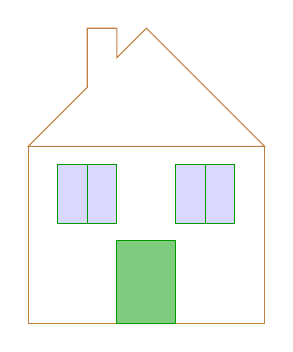
\begin{tikzpicture}[scale = 1.5]
      \draw[brown] (0, 0) -- (0.5, 0.5) -- (0.5, 1) -- (0.75, 1) -- (0.75, 0.75) -- (1, 1) -- (2, 0) -- cycle;
      \draw[brown] (0, 0) -- (0, -1.5) -- (2, -1.5) --  (2, 0);
      \draw[color = green!60!black, fill = blue, fill opacity = 0.15] (0.25, -0.65) rectangle (0.75, -0.15);
      \draw[color = green!60!black, fill = blue, fill opacity = 0.15] (1.25, -0.65) rectangle (1.75, -0.15);
      \draw[color = green!60!black] (0.5, -0.65) -- (0.5, -0.15);
      \draw[color = green!60!black] (1.5, -0.65) -- (1.5, -0.15);
      \filldraw[color = green!60!black, fill opacity = 0.5] (0.75, -1.5) rectangle (1.25, -0.8);
    \end{tikzpicture}}
  \subfigure[subfigure 3]{\label{fig:subfig3}
    
\includegraphics[scale = 0.3]{Pastry_Bag.png}
    }
  \caption[Dessins]{Subfigure 1 \ref{fig:subfig1} et subfigure 2 \ref{fig:subfig2}.}
  \label{fig:figure1}
\end{figure}

La figure \ref{fig:figure1} est vraiment magnifique. Elle est composée des sous-figures \ref{fig:subfig1}, \ref{fig:subfig2} et \ref{fig:subfig3}.

%%%%%%%%%%%%%%%%%%%%%%%%%%%%%
\section{Section 2}
%%%%%%%%%%%%%%%%%%%%%%%%%%%%%

\begin{algorithm}
  \begin{algorithmic}
    \STATE tableau d'entiers tab \COMMENT{tableau d'entiers}
    \STATE int $i$ \COMMENT{indice de parcours}
    \STATE int $m$ \COMMENT{valeur maximale du tableau}
    \STATE
    \STATE $m \leftarrow$ tab[1]
    \FOR{$i$ \FROM 2 \TO length(tab)}
      \IF{$m <$ tab[$i$]}
        \STATE $m \leftarrow$ tab[$i$]
      \ENDIF
      \STATE
      \STATE \PRINT "Le maximum est " + $m$
      \RETURN $m$
    \ENDFOR
  \end{algorithmic}
  \caption[Algorithme 1 (nom dans la liste des algorithmes)]{Met dans $m$ la valeur maximale du tableau tab.\label{ag:algo1}}
\end{algorithm}

L'algorithme \ref{ag:algo1} utilise le package \texttt{algorithmic} dont la francisation des termes se trouve dans le fichier \texttt{algo.sty}.

\begin{algorithm}
  \begin{C}
int max(int* tab, int n) {
  int i; // indice de parcours
  int m; // valeur maximale du tableau
  
  m = tab[0];
  for (i = 1; i < n; i++) {
    if (m < tab[i]) {
      m = tab[i];
    }
  }
  
  printf("Le maximum est %d", m),
  return m;
}
  \end{C}
  \caption[Algo en C]{Retourne la valeur maximale du tableau tab.\label{ag:algoc}}
\end{algorithm}

\begin{algorithm}
  \begin{PseudoCode}
max(tableau d'entiers tab, entier n) {
  entier i // indice de parcours
  entier m // valeur maximale du tableau
  
  m <- tab[1]
  for i from 2 to n {
    if (m < tab[i]) {
      m <- tab[i]
    }
  }
  
  print("Le maximum est ", m),
  return m;
}
  \end{PseudoCode}
  \caption[Algo en PseudoCode]{Retourne la valeur maximale du tableau tab.\label{ag:algop}}
\end{algorithm}

\begin{algorithm}
  \begin{Java}
int max(int[] tab, int n) {
  int i; // indice de parcours
  int m; // valeur maximale du tableau
  
  m = tab[0];
  for (i = 1; i < n; i++) {
    if (m < tab[i]) {
      m = tab[i];
    }
  }
  
  System.out.println("Le maximum est " + m),
  return m;
}
  \end{Java}
  \caption[Algo en Java]{Retourne la valeur maximale du tableau tab.\label{ag:algoj}}
\end{algorithm}

Les algorithmes \ref{ag:algoc} en C, \ref{ag:algop} en pseudo code, et \ref{ag:algoj} en Java utilisent le package \texttt{lstlistings}. La coloration sintaxique utilise les couleurs définies dans le fichier \texttt{couleurs.sty} et les mot-clés se trouvent dans le fichier \texttt{colorationSyntaxique.sty}. Vous pouvez modifier le fichier \texttt{colorationSyntaxique.sty} pour ajouter de nouveaux mot-clés ou y ajouter un langage, pour le moment seuls C, Java, Python, Shell, R et un pseudo code sont disponibles.

%%%%%%%%%%%%%%%%%%%%%%%%%%%%%
\section{Section 3}
%%%%%%%%%%%%%%%%%%%%%%%%%%%%%

La section 3.

%%%%%%%%%%%%%%%%%%%%%%%%%%%%%
\section{Conclusion}
%%%%%%%%%%%%%%%%%%%%%%%%%%%%%
% !TEX root = ../sommaire.tex

\chapter{Chapitre 5}

\chaptoc

\tikzstyle{nodedefault} = [draw, circle]
\tikzstyle{edgedefault} = [draw]

\tikzstyle{n1} = [nodedefault]
\tikzstyle{n2} = [nodedefault]
\tikzstyle{n3} = [nodedefault]
\tikzstyle{n4} = [nodedefault]
\tikzstyle{n5} = [nodedefault]
\tikzstyle{n6} = [nodedefault]
\tikzstyle{n7} = [nodedefault]
\tikzstyle{n8} = [nodedefault]
\tikzstyle{n9} = [nodedefault]

\tikzstyle{a12} = [edgedefault]
\tikzstyle{a13} = [edgedefault]
\tikzstyle{a25} = [edgedefault]
\tikzstyle{a34} = [edgedefault]
\tikzstyle{a46} = [edgedefault]
\tikzstyle{a56} = [edgedefault]
\tikzstyle{a67} = [edgedefault]
\tikzstyle{a68} = [edgedefault]
\tikzstyle{a79} = [edgedefault]
\tikzstyle{a89} = [edgedefault]

% style pour les noeuds roses
\tikzstyle{nrose} = [pink]

% style pour les noeuds bleus
\tikzstyle{nbleu} = [white, fill = bleu]

%%%%%%%%%%%%%%%%%%%%%%%%%%%%%
\section{Section 1}
%%%%%%%%%%%%%%%%%%%%%%%%%%%%%

\begin{figure}
  \centering
    
  \begin{tikzpicture}[every node/.style = {nodedefault}, every path/.style = {edgedefault}] 
    
%%% Définition du graphe %%%

%% Les noeuds
\node[n1] (1) at (0, 0) {NCE};
\node[n2, above right = of 1] (2) {CDG};
\node[n3, below right = of 1] (3) {YUL};
\node[n4, right = of 2] (4) {4};
\node[n5, right = of 3] (5) {5};
\node[n6, below right = of 4] (6) {6};
\node[n7, above right = of 6] (7) {7};
\node[n8, below right = of 6] (8) {8};
\node[n9, below right = of 7] (9) {9};

%% Les arêtes
\path[a12] (1) -- (2);
\path[a13] (1) -- (3);
\path[a25] (2) -- (5);
\path[a34] (3) -- (4);
\path[a46] (4) -- (6);
\path[a56] (5) -- (6);
\path[a67] (6) -- (7);
\path[a68] (6) -- (8);
\path[a79] (7) -- (9);
\path[a89] (8) -- (9);
  \end{tikzpicture}
    
  \caption{Graphe de départ}
  \label{fig:graphe}
\end{figure}

La figure \ref{fig:graphe} est vraiment magnifique.

%%%%%%%%%%%%%%%%%%%%%%%%%%%%%
\section{Section 2}
%%%%%%%%%%%%%%%%%%%%%%%%%%%%%

  \begin{figure}
    \centering
    
    \begin{tikzpicture}[every node/.style = {nodedefault}, every path/.style = {edgedefault}]
      % redéfinitions des nœuds en rose
      \tikzset{n1/.style = nrose}
      \tikzset{n9/.style = nrose}
      
      % et en rectangle
      \tikzset{n2/.style = {rectangle, pink}}
      
      % redéfinitions de nœuds bleus
      \tikzset{n6/.style = nbleu}
      
      % redéfinitions des arêtes
      \tikzset{a12/.style = {->, vert, thick}}
      \tikzset{a25/.style = {-), vert, thick}}
      \tikzset{a56/.style = {-], vert, thick}}
      \tikzset{a67/.style = {(-], vert, thick}}
      \tikzset{a79/.style = {o-[, vert, thick}}
      
      \tikzset{a13/.style = {red, dashed, thick}}
      
      
%%% Définition du graphe %%%

%% Les noeuds
\node[n1] (1) at (0, 0) {NCE};
\node[n2, above right = of 1] (2) {CDG};
\node[n3, below right = of 1] (3) {YUL};
\node[n4, right = of 2] (4) {4};
\node[n5, right = of 3] (5) {5};
\node[n6, below right = of 4] (6) {6};
\node[n7, above right = of 6] (7) {7};
\node[n8, below right = of 6] (8) {8};
\node[n9, below right = of 7] (9) {9};

%% Les arêtes
\path[a12] (1) -- (2);
\path[a13] (1) -- (3);
\path[a25] (2) -- (5);
\path[a34] (3) -- (4);
\path[a46] (4) -- (6);
\path[a56] (5) -- (6);
\path[a67] (6) -- (7);
\path[a68] (6) -- (8);
\path[a79] (7) -- (9);
\path[a89] (8) -- (9);      
    \end{tikzpicture}
    
    \caption{Graphe avec des nœuds en rose et d'autres en bleu}
  \label{fig:grapherb}
  \end{figure}

%%%%%%%%%%%%%%%%%%%%%%%%%%%%%
\section{Section 3}

  \begin{figure}
    \centering
    
    \begin{tikzpicture}[every node/.style = {nodedefault}, every path/.style = {edgedefault}]
      
%%% Définition du graphe %%%

%% Les noeuds
\node[n1] (1) at (0, 0) {NCE};
\node[n2, above right = of 1] (2) {CDG};
\node[n3, below right = of 1] (3) {YUL};
\node[n4, right = of 2] (4) {4};
\node[n5, right = of 3] (5) {5};
\node[n6, below right = of 4] (6) {6};
\node[n7, above right = of 6] (7) {7};
\node[n8, below right = of 6] (8) {8};
\node[n9, below right = of 7] (9) {9};

%% Les arêtes
\path[a12] (1) -- (2);
\path[a13] (1) -- (3);
\path[a25] (2) -- (5);
\path[a34] (3) -- (4);
\path[a46] (4) -- (6);
\path[a56] (5) -- (6);
\path[a67] (6) -- (7);
\path[a68] (6) -- (8);
\path[a79] (7) -- (9);
\path[a89] (8) -- (9);
      
      \tikzset{every node/.style = {}} % on ne veut plus de cercle autour des nœuds
      \node[red] () at ($(1) !.5! (2)$) {toto}; % directement au milieu
      
      \node[bleu, right] () at ($(4) !.35! (6)$) {tata}; % à droite, à 0.35 de (4)
      
      \tikzset{every path/.style = {}} % on ne veut plus dessiner les chemins
      \path (7) -- (9) node [midway, above, sloped, vert] () {titi};
      
      \path (8) -- (9) node [midway, below, sloped, pink] (ici) {ici};
      
      \node[right = 0.5cm, pink] (regardez) at (9 |- 8) {Regardez};  % le nœud se trouve à 0.5cm à droite du point ayant la même abscisse que (9) et la même ordonnée que (8);
      
      \draw[->, pink, very thick] (regardez) -- (ici);

    \end{tikzpicture}
    
    \caption{Graphe de départ avec une étiquette sur certaines arêtes}
  \label{fig:grapheetiq}
  \end{figure}
%%%%%%%%%%%%%%%%%%%%%%%%%%%%%

%%%%%%%%%%%%%%%%%%%%%%%%%%%%%
\section{Conclusion}
%%%%%%%%%%%%%%%%%%%%%%%%%%%%%

% !TEX root = ../sommaire.tex

\chapter{Conclusion et Perspectives}

\section{Conclusion}
Les macarons c'est bon et ceux de Ladurée sont semble-t-il meilleurs. \cite{F2012}

\section{Perspectives}
Encore beaucoup de travail à faire.

\backmatter

\bibliographystyle{plain}
\bibliography{biblio}

\addcontentsline{toc}{section}{Bibliographie} 

\listoffigures
%\listoftables

\renewcommand{\listtheoremname}{Liste des définitions}
\listoftheorems[ignoreall,show={definition}]

\pagestyle{empty}

\renewcommand{\listtheoremname}{Liste des exemples}
\listoftheorems[ignoreall,show={example}]

%\listofalgorithms


\appendix

% !TEX root = ../sommaire.tex

\chapter*{}

%%%%%%%%%%%%%%%%%%%%%%%%%%%%%
\section{Équation}
%%%%%%%%%%%%%%%%%%%%%%%%%%%%%

  $$
  \begin{array}{l c l}
    Z = \min c\cdotp x & & Z_{LR}(\lambda) = \min c\cdotp x + \lambda^T\cdotp(b_h - A_hx)\\
    \mbox{s.t. }
      \left\{
        \begin{array}{l}
          A_hx \geq b_h\\
          A_ex \geq b_e\\
          x \in \{0, 1\}
        \end{array}
      \right.
    & \longrightarrow
    & \mbox{s.t. }
      \left\{
        \begin{array}{l}
          A_ex \geq b_e\\
          x \in \{0, 1\}
        \end{array}
      \right.
  \end{array}
  $$
  
  
\begin{figure}
  \caption{Figure vide}
\end{figure}


%%%%%%%%%%%%%%%%%%%%%%%%%%%%%
\section{Cosinus}
%%%%%%%%%%%%%%%%%%%%%%%%%%%%%

\def\b#1{\textcolor{bleu}{#1}}
\def\v#1{\textcolor{violet}{#1}}
\def\r#1{\textcolor{pink}{#1}}
\def\o#1{\textcolor{orange}{#1}}
\def\g#1{\textcolor{vert}{#1}}

\begin{figure}
  \begin{tikzpicture}
    \draw[->, black!50] (0, -1.5) -- (0, 1.5);
    \draw[->, black!50] (-1.5, 0) -- (1.5, 0);
    \begin{scope}[thick, bleu]
      \clip (0, 0) rectangle (1.5, 1.5);
      \draw (0, 0) circle (1);
      \draw (0.5, 0.5) node {1};
    \end{scope}
    \begin{scope}[thick, pink]
      \clip (0, 0) rectangle (-1.5, 1.5);
      \draw (0, 0) circle (1);
      \draw (-0.5, 0.5) node {2};
    \end{scope}
    \begin{scope}[thick, violet]
      \clip (0, 0) rectangle (-1.5, -1.5);
      \draw (0, 0) circle (1);
      \draw (-0.5, -0.5) node {3};
    \end{scope}
    \begin{scope}[thick, orange]
      \clip (0, 0) rectangle (1.5, -1.5);
      \draw (0, 0) circle (1);
      \draw (0.5, -0.5) node {4};
    \end{scope}
  \end{tikzpicture}
  \begin{tikzpicture}[xscale = 1.25]
    \draw[->, black!50] (0, -1.5) -- (0, 1.5);
    \draw[->, black!50] (-0.5, 0) -- (8.5, 0);
    \draw[dotted] (1, -1.5) -- (1, 1.5);
    \draw[dotted] (2, -1.5) -- (2, 1.5);
    \draw[dotted] (3, -1.5) -- (3, 1.5);
    \draw[dotted] (4, -1.5) -- (4, 1.5);
    \draw[dotted] (5, -1.5) -- (5, 1.5);
    \draw[dotted] (6, -1.5) -- (6, 1.5);
    \draw[dotted] (7, -1.5) -- (7, 1.5);
    \begin{scope}[thick, bleu]
      \clip (0, 1.5) rectangle (1, -1.5);
      \draw (0, 1) cos (1, 0) sin (2, -1) cos (3, 0) sin (4, 1);
      \draw (0.5, 0) node {1};
    \end{scope}
    \begin{scope}[thick, pink]
      \clip (1, 1.5) rectangle (2, -1.5);
      \draw (0, 1) cos (1, 0) sin (2, -1) cos (3, 0) sin (4, 1);
      \draw (1.5, 0) node {2};
    \end{scope}
    \begin{scope}[thick, violet]
      \clip (2, 1.5) rectangle (3, -1.5);
      \draw (0, 1) cos (1, 0) sin (2, -1) cos (3, 0) sin (4, 1);
      \draw (2.5, 0) node {3};
    \end{scope}
    \begin{scope}[thick, orange]
      \clip (3, 1.5) rectangle (4, -1.5);
      \draw (0, 1) cos (1, 0) sin (2, -1) cos (3, 0) sin (4, 1);
      \draw (3.5, 0) node {4};
    \end{scope}
    
    \begin{scope}[xshift = 4cm]
    \begin{scope}[thick, bleu]
      \clip (0, 1.5) rectangle (1, -1.5);
      \draw (0, 1) cos (1, 0) sin (2, -1) cos (3, 0) sin (4, 1);
      \draw (0.5, 0) node {1};
    \end{scope}
    \begin{scope}[thick, pink]
      \clip (1, 1.5) rectangle (2, -1.5);
      \draw (0, 1) cos (1, 0) sin (2, -1) cos (3, 0) sin (4, 1);
      \draw (1.5, 0) node {2};
    \end{scope}
    \begin{scope}[thick, violet]
      \clip (2, 1.5) rectangle (3, -1.5);
      \draw (0, 1) cos (1, 0) sin (2, -1) cos (3, 0) sin (4, 1);
      \draw (2.5, 0) node {3};
    \end{scope}
    \begin{scope}[thick, orange]
      \clip (3, 1.5) rectangle (4, -1.5);
      \draw (0, 1) cos (1, 0) sin (2, -1) cos (3, 0) sin (4, 1);
      \draw (3.5, 0) node {4};
    \end{scope}
    \end{scope}
  \end{tikzpicture}
  \caption{Cosinus}
\end{figure}
  
  
  $\cos([x^-, x^+]) = [-1, 1]$ si $x^+ - x^- \geq 2\pi$
  
  sinon
  
  $\begin{array}{c | c | l}
  x^- \mod 2\pi \in & x^+ \mod 2\pi \in & \cos([x^-, x^+])\\\hline
  1 & 1 & \left\{\begin{array}{ll}\b{[\cos(x^+), \cos(x^-)]} & \mbox{si } x^- \mod 2\pi \leq x^+ \mod 2\pi\\\o{[-1, 1]} & \mbox{sinon}\end{array}\right.\\
  1 & 2 & \b{[\cos(x^+), \cos(x^-)]}\\
  1 & 3 & \r{[-1, \cos(x^-)]}\\
  1 & 4 & \r{[-1, \max(\cos(x^-), \cos(x^+))]}\\[5pt]
  
  2 & 1 & \o{[-1, 1]}\\
  2 & 2 & \left\{\begin{array}{ll}\b{[\cos(x^+), \cos(x^-)]} & \mbox{si } x^- \mod 2\pi \leq x^+ \mod 2\pi\\\o{[-1, 1]} & \mbox{sinon}\end{array}\right.\\
  2 & 3 & \r{[-1, \max(\cos(x^-), \cos(x^+))]}\\
  2 & 4 & \r{[-1, \cos(x^+)]}\\[5pt]
  
  3 & 1 & \v{[\cos(x^-), 1]}\\
  3 & 2 & \v{[\min(\cos(x^-), \cos(x^+)), 1]}\\
  3 & 3 & \left\{\begin{array}{ll}\g{[\cos(x^-), \cos(x^+)]} & \mbox{si } x^- \mod 2\pi \leq x^+ \mod 2\pi\\\o{[-1, 1]} & \mbox{sinon}\end{array}\right.\\
  3 & 4 & \g{[\cos(x^-), \cos(x^+)]}\\[5pt]
  
  4 & 1 & \v{[\min(\cos(x^-), \cos(x^+)), 1]}\\
  4 & 2 & \v{[\cos(x^+), 1]}\\
  4 & 3 & \o{[-1, 1]}\\
  4 & 4 & \left\{\begin{array}{ll}\g{[\cos(x^-), \cos(x^+)]} & \mbox{si } x^- \mod 2\pi \leq x^+ \mod 2\pi\\\o{[-1, 1]} & \mbox{sinon}\end{array}\right.\\
  \end{array}$

%%%%%%%%%%%%%%%%%%%%%%%%%%%%%
\section{Section C}

\begin{definition}[test definition]
  Ceci est une définition
\end{definition}

\begin{example}[test exemple]
  Ceci est un exemple
\end{example}

%%%%%%%%%%%%%%%%%%%%%%%%%%%%%

%%%%%%%%%%%%%%%%%%%%%%%%%%%%%
\section{Conclusion}
%%%%%%%%%%%%%%%%%%%%%%%%%%%%%

\end{document}
